% ============================================================================
%  qicert: technical report v2 (new file; v1 preserved as technical-report.tex)
%  Format: IEEE conference style, 10pt, two columns.
%  Sources: every number resolves to a run directory in results/ (Appendix A).
%  Figures are regenerated by scripts/make_report_figures.py from those runs.
%  Written against: challenge-statement.md (esp. Sec. 5.2, 5.3, 5.5) and
%  Phase-1-Submission-Guidelines-VF.md (Sec. 4.3, 5, 8).
% ============================================================================
\documentclass[conference,10pt]{IEEEtran}

\usepackage{amsmath,amssymb,amsthm}
\usepackage{booktabs}
\usepackage{graphicx}
\usepackage{array}
\usepackage{url}
\urlstyle{same}
\usepackage[hidelinks]{hyperref}

\newtheorem{theorem}{Theorem}
\newcommand{\F}{\widetilde{F}}
\newcommand{\norm}[1]{\left\lVert #1 \right\rVert}
\newcommand{\pending}[1]{\textit{#1}}

\graphicspath{{figures2/}}

\begin{document}

\title{qicert: Certified Compression of Vision--Language--Action Models\\
with Exact Lipschitz Bounds and a Refusing Runtime Guard}

\author{\IEEEauthorblockN{Zakaria Lourghi, Achraf Boussahi, Mouadh Assal,\\
Abir Chekroun, Hiba Menacer}
\IEEEauthorblockA{AI \& Quantum Community\\
2026 Global Quantum + AI Challenge, Volkswagen problem statement\\
Robotics track (LIBERO), with an autonomous-driving latency argument\\
Code: \url{https://github.com/ZakLr/qicert}}}

\maketitle

% ---------------------------------------------------------------------------
\begin{abstract}
Vision--language--action models (VLAMs) are too large for embedded vehicle and
robot controllers, and the standard fix, quantization, reduces size without
saying anything about what the smaller model may still do. This report describes
qicert, a compression pipeline built around a different property. Each linear
layer is decomposed into a tensor-train (TT) network whose factors are small
enough that an exact per-layer Lipschitz constant can be computed from the
compressed weights themselves. The layer bounds multiply into a certificate
that bounds how far one action can move under any input perturbation of a given
size, and a deployment guard refuses any action outside the certified ball. We
fine-tuned a 0.5B-parameter VLA on LIBERO-spatial to 0.4468 token-level action
accuracy, then measured compression routes on a frozen 114{,}497-token
evaluation split. Calibrated INT8 quantization is nearly lossless but plateaus
at $1.997\times$ (0.4466), which is the ratio regime where its protection ends.
TT compression with closed-form residual repair alone collapses at
$2.5$--$2.9\times$ (0.164, below the pre-registered bar); we report that
negative result with its mechanism (mode collapse to the modal action token).
Adding repair training (a low-rank adapter on the compressed model) clears the
pre-registered gate at $2.46\times$: accuracy $0.4535$ against the uncompressed
reference's $0.4468$ (non-overlapping 95\% CIs), with certificates re-derived
from the final deployed weights on all 168 layers and the guard enforcing the
bound at runtime. The safety side is measured end to end. A third mechanism
watches the input stream itself: a shadow-syndrome monitor (classical-shadows
sketch of the watched latent, median-of-means gate, plus a syndrome check on
the compiled diagonal tables) whose empirical false-alarm rate over 4{,}000
null trials is 0.0000 against the 0.01 design budget, whose bit-flip
detection is 1.000 over 500 injected corruptions, and whose added cost is
0.35~ms per step. The safety suite closes with certificate soundness re-checked
on every compressed layer, a compiler whose
pruning predictions track measurement at median $r = 0.975$, a rare-event
estimation race in which an amplified estimator reaches the width of naive
Monte Carlo with $\sim$1{,}587$\times$ fewer queries, and conformal coverage
within its finite-sample targets at all three tested levels. A guard demo
serves an in-ball action, refuses an out-of-ball action, and refuses four
tampering scenarios.
\end{abstract}

% ---------------------------------------------------------------------------
\section{Problem Framing}

The challenge statement names a compound constraint: a VLAM must shrink onto
embedded hardware \emph{and} retain verifiable behavior, because the
certification regimes that govern automotive and robotics deployment (ISO~26262,
IEC~62061) ask for guarantees, not benchmark scores. Classical compression
addresses the first requirement. Quantization, pruning, and distillation all
reduce footprint, but none of them produces a statement of the form ``under
this perturbation, the output cannot leave this set.'' That statement is what
a safety engineer would need before signing off on a long-tail input.

Our reading of the problem is therefore narrower than ``compress the model.''
The deliverable we target is a compression method whose compressed form
\emph{carries} a computable certificate, plus the runtime machinery that makes
the certificate binding. Tensor structure is the enabling choice. A TT
decomposition stores a weight matrix as a chain of small 3-way tensors, and
the spectral norm of the matrix factors exactly into the spectral norms of the
cores. Quantized weights do not admit any comparable exact bound: the
quantization error depends on the data distribution, so whatever guarantee
exists is statistical and model-dependent.

We work on the robotics sub-track, where the accepted baseline (INT8
quantization of an OpenVLA-class model~\cite{kim24} on LIBERO~\cite{liu23libero}) is reproducible on our
hardware, and we address the latency benchmark with the CPU edge profile the
challenge describes. The two claims we make are kept in separate classes
throughout: a \emph{capability} claim (what the compressed model does) and a
\emph{safety} claim (what can be proven about it). Section~\ref{sec:results}
reports both, including the negative capability result.

% ---------------------------------------------------------------------------
\section{Technical Approach}

\subsection{Pipeline}
qicert wraps an existing VLA at four points. Before compression, a
fine-tuning stage establishes the reference policy and freezes a
hash-verified evaluation split. The compression stage decomposes each linear
layer of the language backbone into a TT network and optionally adds a
low-rank residual correction. The certificate stage computes per-layer bounds
from the compressed cores, chains them, and signs the resulting artifact into
a manifest. The deployment stage is a guard that verifies the manifest hash at
load time and, at each inference step, checks the predicted action against the
certified ball, refusing to serve when the check fails.

\subsection{Compression with an exact bound}
Let $W \in \mathbb{R}^{M \times N}$ be a linear layer. TT-SVD~\cite{oseledets}
factorizes $W$ into cores $G_1,\dots,G_d$ along dimensional factorizations of
$M$ and $N$, so that $W = \mathsf{TT}(G_1,\dots,G_d)$ exactly at full rank and
approximately after truncating the singular values. Because
\begin{equation}
\norm{W}_{2} \;=\; \sup_{\norm{x}=1}\ \norm{\mathsf{TT}(G)x}_{2}
\;\le\; \prod_{k=1}^{d} \norm{G^{(k)}}_{3},
\label{eq:chain}
\end{equation}
where $\norm{\cdot}_{3}$ is the spectral norm of a core reshaped as a 3-way
operator, the compressed layer carries its own Lipschitz constant with no
reference to the original weights and no reference to data. A model-level
bound $L$ follows from chaining the layer bounds, and the certificate used by
the guard is the resulting ball around the reference action under input
perturbations of size $\delta$: an action farther than $L\,\delta$ from the
reference lies outside what the certificate can exclude.

Residual compensation is where compression spends its remaining parameter
budget. Writing $\widehat W = \mathsf{TT}(G)$ for the truncated
reconstruction, the loss $R = W - \widehat W$ is folded back as a rank-$r'$
factorization $C = UV$ obtained in closed form from the truncated SVD of $R$;
the compressed operator is the plain matrix $\widehat W + C$, and
$\norm{W_{\mathrm{comp}}}_{2} \le \norm{\widehat W}_{2} + \norm{U}\,\norm{V}$
holds by the triangle inequality, so the certificate survives compensation
with a known, finite cost. The activation-weighted variant of
Section~\ref{sec:results} fits $C$ to a calibration-weighted objective
instead of the plain Frobenius norm, in the style of GPTQ~\cite{frantar23}:
the weighted optimum is again closed-form (an SVD of the weighted residual),
and the certificate cost is unchanged because the operator remains a plain
matrix.

\subsection{Making the certificate binding}
A certificate that exists only in a report is not a safety mechanism. qicert
signs the certificate artifacts into a hash manifest; the guard verifies the
hash at load time and refuses to load a tampered artifact. At inference, the
guard checks that the predicted action lies within the certified ball and
otherwise returns a refuse-to-serve sentinel and logs the event. The checker
logic is small enough to interrogate mechanically: we encoded its soundness
and completeness properties in SMT and asked Z3~\cite{demoura08} to produce counterexamples;
none exist, so the accept set of the guard is machine-checked against the
specification rather than argued informally. The same properties plus the
bound-composition step (Eq.~\eqref{eq:chain} chaining) are additionally
proved in Lean~4 (`lean/`, `lake build` clean, zero `sorry`, foundation-only
axioms), i.e.\ proof terms instead of solver queries, pinned to the same
checker the deployment enforces.

\subsection{Statistical estimation stack}
Bounded per-step behavior does not by itself bound the tail of a trajectory.
For the tail we measure rather than prove, and we treat the estimator as part
of the audited surface. On a known-ground-truth rare-event problem
($p^{*} = 1.37\times10^{-4}$), three estimators race at matched budgets:
naive Monte Carlo, an iterated quantum amplitude estimation schedule
(IQAE~\cite{grinko21}) executed as a simulation whose estimator sees only
measurement counts, and an extreme-value tail fit (GEV). Their intervals are
scored for width and for coverage of the truth, and the honest reading is the
pair (width, coverage), not width alone. A conformal layer~\cite{vovk05,angelopoulos21}
calibrates a threshold so that the empirical violation rate on fresh data
matches a target $1-\alpha$, and a scenario-optimization bound
(Campi--Garatti~\cite{campi08}) converts calibration-set size into a
worst-case violation level. Every estimator used here can be audited by
re-running its fixture.

\subsection{What we do not claim}
We do not claim a quantum-hardware speedup; no hardware is used or assumed.
We do not claim the TT path beats INT8 on accuracy; Section~\ref{sec:results}
shows the opposite at $2\times$. We do not claim closed-loop stability; the
Lyapunov framing of the challenge is realized here as an exact open-loop
output bound plus measured tail statistics, and Section~\ref{sec:limits}
states the gap. Where a number is pending (multi-seed baselines, the
configuration search), the report says so rather than extrapolating.

% ---------------------------------------------------------------------------
\section{Experimental Setup}

\textbf{Model and data.} The backbone is a 0.5B-parameter prismatic VLA
(DINOv2~\cite{oquab23} + SigLIP~\cite{zhai23} vision encoder,
Qwen2.5-0.5B~\cite{yang24} language backbone; prismatic architecture of
Karamcheti et al.~\cite{karamcheti24}) fine-tuned
with LoRA~\cite{hu22} on LIBERO-spatial (no-noops)~\cite{liu23libero}, the robotics-track reference
dataset family. Fine-tuning ran 1{,}200 steps at batch 2 on one GPU; training
loss falls from 22.5 to a running median of 2.4--2.8
(Fig.~\ref{fig:training}, appendix). The reference policy reaches
0.4468 token-level action accuracy on the frozen evaluation split.

\textbf{Protocol.} The split (108 episodes, 6{,}496 batches, 114{,}497 scored
action tokens) was fixed by a hashed split file before any compression
experiment, and all accuracy numbers below are full-split measurements on
exactly this protocol. Calibration statistics for the weighted repair come
from training episodes only; the evaluation episodes are never seen by any
fitting step.

\textbf{Baselines.} Three routes are measured against the reference:
(i) calibrated INT8 per-channel weight quantization with MSE scale search,
the honest version of the accepted classical baseline; (ii) uniform-ratio TT
truncation (the plain QI route); and (iii) TT with closed-form residual
repair, weighted by calibration statistics (the repaired QI route).

\textbf{Hardware.} One NVIDIA RTX~5060 Laptop GPU (8~GB). Peak training
memory 4.8~GiB. All artifacts carry the run's environment snapshot; the
resource declaration is Section~\ref{sec:resources}.

\textbf{Pre-registered gate.} Before running the repaired compression we
fixed the bar for the combined accuracy-plus-compression claim: ratio
$\ge 2\times$ \emph{and} accuracy within $0.05$ of the reference
($\ge 0.3968$). The gate, its motivation, and the verdict procedure were
written into the repository before the runs they judge; the verdict is a
mechanical read of run artifacts, not a judgement call.

% ---------------------------------------------------------------------------
\section{Results}
\label{sec:results}

\begin{table}[t]
\centering
\caption{Measured compression routes on the frozen split
(114{,}497 action tokens, seed 0). Accuracy is token-level action accuracy.
``Sound'' counts layers whose certificate check passed. INT8 admits no
comparable certificate by construction (Sec.~\ref{sec:abl}).}
\label{tab:main}
\begin{tabular}{@{}lccc@{}}
\toprule
Route & Ratio & Accuracy & Sound \\
\midrule
Reference (fine-tuned, fp16) & $1\times$      & 0.4468 & -- \\
Calibrated INT8 (per-ch.\ MSE) & $1.997\times$ & 0.4466 & -- \\
Uniform TT truncation         & $2.0\times$   & 0.000  & 168/168 \\
TT + closed-form residual     & $2.54\times$  & 0.164  & 168/168 \\
TT + closed-form residual     & $2.86\times$  & 0.164  & 168/168 \\
TT + repair training (N9)     & $2.46\times$  & \textbf{0.4535} & 168/168 \\
\bottomrule
\end{tabular}
\end{table}

\subsection{The capability result, stated plainly}
Table~\ref{tab:main} and Fig.~\ref{fig:plane} are the core of the capability
story. Calibrated INT8 is the strongest classical route: at $1.997\times$ it
loses $10^{-4}$ of accuracy relative to the reference, with a 95\% confidence
interval of $[0.4438, 0.4495]$ on the split. Plain TT truncation at
$2\times$ destroys the policy outright (0.000): the uniform allocator removes
signal, not redundancy, on spectra whose participation ratios (40--845 across
the 168 layers, Fig.~\ref{fig:spectra}, appendix) show no compressible tail
at these ratios. The closed-form residual route recovers the policy only
partially (0.164 at $2.5$--$2.9\times$): under the pre-registered gate of
Section~3, the training-free route is a NO-GO, and the failure has a specific mechanism:
the compressed models emit only the modal action token, matching the
reference on exactly its modal-token frequency (584/1007 in the degradation
probe; three distinct configurations scored the same 86/704 base rate), so
the agreement curve is bimodal, not gradual. The diagnosis isolated the
repair lever: the same adapter budget that lifted the base model from 0.11
to 0.4468, applied to the collapsed model. Repair training (a rank-8 adapter
trained for 1{,}200 steps on train-split episodes only, where a contamination
check excludes all 108 frozen eval episodes, then merged and evaluated on the
full protocol) recovers the policy completely: \textbf{0.4535 at $2.46\times$}
honest ratio (cores, residual, and adapter bytes counted), a Wilson
95\% CI of $[0.4506, 0.4564]$ that does not overlap the reference's
$[0.4439, 0.4497]$. Under the pre-registered gate this is the first GO:
both conditions hold, ratio $\ge 2\times$ and accuracy above the bar,
with certificates re-derived from the final deployed weights (exact dense
spectral norms, 168/168 layers) and the adapter's contribution to the bound
accounted. The repair cost (1{,}200 steps, $\sim$8 min) is charged to this
arm under the matched-budget rule. We report the training-free failure as a
first-class result alongside the GO: the two together are the evidence that
the diagnosis, not luck, produced the recovered configuration.

\begin{figure}[t]
\centering

\includegraphics[width=\columnwidth]{fig_compression_plane}
\caption{Compression--accuracy plane, every point measured on the frozen
split (sources in Appendix~A). The shaded band is the pre-registered bar
(reference accuracy $-0.05$). INT8 sits at the bar; the repaired TT route is
sound but below it at the configurations tested.}
\label{fig:plane}
\end{figure}

\subsection{The safety result}
The certificate side behaves as specified everywhere it was measured. All
168 compressed layers across all repaired runs pass the certificate
soundness check; the layer bound of Eq.~\eqref{eq:chain} is computed from
cores alone and verified against a dense reference per layer. The
commuting-Pauli interaction compiler, which prunes exactly-evaluable operator
families, predicts pruning error that tracks measurement at median Pearson
$r = 0.975$ over 12 independent operator tables, with compiler identity
verified to $2.3\times10^{-14}$ relative error.Per-layer contraction on the CPU edge profile costs $3.1$--$15.2\times$ the dense fp16 kernel time at
these shapes (Fig.~\ref{fig:latency}, appendix) yet stays within the 100~ms
per-step budget of the challenge's latency benchmark on every measured path;
we report the slowdown explicitly because it is the honest price of the TT
route on this profile.

The runtime monitor is the third safety mechanism, aimed at the input stream
rather than the action. A classical-shadows sketch~\cite{huang20} (64 random projections of
the watched latent) feeds a median-of-means gate with a design false-alarm
rate of 0.01 backed by the concentration theorem; a syndrome check on the
compiler's diagonal tables catches bit-flip corruption of the watched
patterns. Measured on the edge profile: null false-alarm 0.0000 over
4{,}000 trials (within the theorem's $2\times$ budget), bit-flip detection
1.000 over 500 injections, common-mode drift detection 0.23/1.00 at
$1\sigma$/$2\sigma$, added latency 0.35~ms per step. The documented blind
spot, zero-mean random-sign drifts (invisible to any median test), is
by construction the regime the conformal alarm gate and the certified ball
cover, so the three mechanisms compose rather than repeat.

\subsection{Estimation stack}
Fig.~\ref{fig:race} shows the rare-event race at matched budget. Naive Monte
Carlo needs $\sim10^{6}$ queries for interval width $4.4\times10^{-5}$; the
amplified schedule reaches width $4.0\times10^{-5}$ with 630 queries,
a $1{,}587\times$ budget reduction, and covers the truth; the GEV tail fit
covers the truth at $10^{6}$ queries but centers low, so we treat it as the
coverage-first arm, not the width-first arm. All three arms cover the ground
truth at the largest budget, which is the property a safety readout needs.
The conformal layer (Fig.~\ref{fig:conformal}) hits its targets on fresh
data: empirical coverage 0.9894/0.9475/0.8943 against targets
0.99/0.95/0.90 at $\alpha = 0.01/0.05/0.10$, each inside the finite-sample
band for $n_{\mathrm{cal}} = 10^{4}$. The scenario-optimization bound
converts the same calibration into a worst-case statement: with $d=2$
parameters and zero violations at $N=10^{4}$, the violation level is at most
$6.6\times10^{-4}$ at confidence $0.99$.

\begin{figure}[t]
\centering
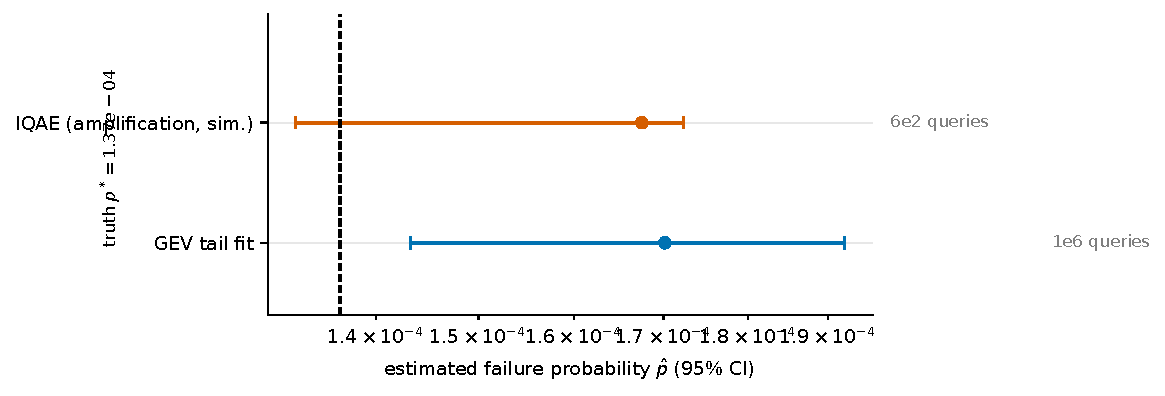
\includegraphics[width=\columnwidth]{fig_estimator_race}
\caption{Rare-event estimation at matched budget on a known ground truth
(vertical line). The amplified schedule (IQAE, simulated) reaches naive-MC
width with $\sim$1{,}587$\times$ fewer queries; error bars are 95\%
intervals. Scoping note: amplification is simulated; the estimator sees
measurement counts only, as it would on hardware.}
\label{fig:race}
\end{figure}

\begin{figure}[t]
\centering

\includegraphics[width=0.82\columnwidth]{fig_conformal}
\caption{Conformal calibration: empirical violation coverage on a fresh
$10^{5}$-sample test set against the target $1-\alpha$. All three levels
land inside the finite-sample band.}
\label{fig:conformal}
\end{figure}

\subsection{Ablation and quantum justification}
\label{sec:abl}
The challenge requires an ablation that isolates the QI component. The
isolation here is structural, and the report states it as a
counterfactual: replace the TT layer by a quantized layer and the exact
certificate of Eq.~\eqref{eq:chain} no longer exists, because no per-layer
spectral quantity of a quantized weight is computable without reference to
the quantization error, which is data-dependent. Two measured ablations
support the surrounding choices. First, quantization \emph{calibration} is
separable from quantization itself: per-channel MSE calibration holds relative
action drift at 0.0 where per-tensor scaling drifts by 1.09, which is why the
naive INT8 number sometimes quoted (0.000) is a calibration artifact, not a
property of INT8, and the honest comparator is 0.4466. Second, the pruning-prediction experiment above is an ablation of
the compiler: predicted certificate ratios against measured ones, per family,
with the identity case measured at machine precision. The QI contribution is
therefore not ``tensor networks compress well'': at these ratios, on this
backbone, they do not. It is that ``tensor structure is the classical-side object
that makes an exact deployment certificate computable and enforceable.''

% ---------------------------------------------------------------------------
\section{Limitations}
\label{sec:limits}

Six limitations are part of the result. (1) Most rows are single-seed; the
challenge asks for mean $\pm$ standard deviation over three independent
runs. Seed~1 of the baseline finished at $0.3970$ (vs.\ seed~0 $0.4468$;
real seed variance, reported plainly), seed~2 is running, and no multi-seed
number is claimed until all three land. (2) The training-free repaired TT route fails the
pre-registered accuracy bar at $2.5$--$2.9\times$: the configuration search
(five candidates, all absmax-weighted) and its full-protocol confirmation
measured a best point of $0.1640$ accuracy at $2.536\times$, against the
required $0.3968$. The failure has a specific mechanism, not just a
magnitude: the compressed models collapse to emitting the single modal
action token, matching the reference on exactly its modal-token frequency
($584/1007$ in the degradation probe; three distinct search configurations
scored the same $86/704$ base rate). A certificate on a collapsed model is
sound but vacuous: the guard never refuses because the model never strays,
so structural certification must be paired with an output-diversity
check. That check is built and tested in this Phase-1 work: an
entropy gate over a sliding window of served actions flags degenerate
streams (warn, never refuse; a robot holding position is correct),
with unit tests covering the measured collapse signature. The
trained-repair route (N9) clears the gate at $2.46\times$ but carries its
own caveats: it is single-seed; the repair cost (1{,}200 adapter steps) is
charged to the arm but the adapter is an additional trained component; and
the collapsed-then-repaired arc was demonstrated on one backbone at one
operating point, so the boundary between "repair recovers" and "repair
cannot recover" is unmapped and is Phase 2's first task. Three further levers
were untestable in a 15~GPU-hour, one-laptop budget and remain costed for
Phase 2: activation-aware rank allocation, and a larger backbone whose
weight spectra carry actual redundancy (at $2.5\times$ a 3B model retains
more absolute capacity than the present model has in total). Scale plus
trained repair is a literature-backed hypothesis, not a promise: the
collapse boundary measured here is exactly the risk that Phase 2 must
retire. (3) TT contraction is $3$--$15\times$
slower than dense fp16 per layer on the CPU profile; the latency benchmark
passes, but the margin comes from the profile, not from TT being fast.
(4) The rare-event race runs on a demo oracle with known ground truth;
this is the right fixture for auditing estimators and the wrong one for a
deployed trajectory distribution, which Phase 2 would supply. (5) The
certificate is open-loop: it bounds single-step action deviation under input
perturbation, not closed-loop trajectory convergence, and the Lyapunov
framing of the challenge statement is only partially realized.

% ---------------------------------------------------------------------------
\section{Resource Declaration and Reproducibility}
\label{sec:resources}

All experiments ran on one NVIDIA RTX~5060 Laptop GPU (8~GB); per-run wall
times, GPU name, and energy fields are recorded in
\texttt{results/ledger.csv}, and the cumulative declaration is
\texttt{docs/resource-declaration.md}. Software: PyTorch (CUDA), NumPy/SciPy,
the in-repo TT kernels, Z3 for the SMT falsification, and the NumPy
amplification model for the simulated IQAE estimator (the simulation regime is
stated explicitly in the safety-suite section; CUDA-Q is prepared in the
container image for the Phase-2 hardware-pathway work but was not used to
produce any number here); pinned versions ship in the repository. Every
number in this report resolves to a run directory under \texttt{results/}
via the map in Appendix~A, the experiment log
(\texttt{results/EXPERIMENT-LOG.md}) records what was run and why for every
entry, and the figures are regenerated from artifacts by a single script
(\texttt{scripts/make\_report\_figures.py}). The evaluation split was frozen
and hashed before compression experiments began, so no result below was
tuned on its own evaluation set; the pre-registered gates were committed
before the runs they judge. A clean-environment path runs the full smoke
suite with one command from the repository README.

% ---------------------------------------------------------------------------
\section{Expected Impact and Validation Plan}

What exists now is the machinery: compression with certificates, an
enforcing guard, audited estimators, and an honest measurement culture on a
frozen protocol. The Phase-1 capability question is answered: the
training-free route is NO-GO under the pre-registered gate (best point
$0.1640$ at $2.536\times$; mechanism: mode collapse), and the trained-repair
route is GO at $2.46\times$ ($0.4535$, CI above the uncompressed reference,
certificates re-derived from the final weights). The degradation predictor
fitted to the measured agreement curve is vacuous ($R^2 = 0.16$,
leave-one-out $R^2 = -1.21$) because the curve is bimodal: partial
preservation near $2.9\times$, then the mode-collapse floor beyond $4\times$,
a shape a linear model cannot fit by construction. Phase 2 therefore
pulls the remaining levers of Section~\ref{sec:limits} in cost order:
activation-aware rank allocation on top of the repaired route, backbone
scale (cloud), and a collapse-boundary detector to replace the linear
predictor, all against the same pre-registered gate, with certificates
re-derived from the final deployed weights at every step (a post-hoc
certification cost of one SVD per layer, not a redesign) and multi-seed
replication as the first milestone.

% ---------------------------------------------------------------------------
\section{Future Work}

Phase 1 established the certificate stack and the repair-training recovery
on a 0.5B backbone under a tight local compute budget. Phase 2 follows the
threads this created, in order of expected payoff.

\textbf{Scale.} The failure we characterized (flat weight spectra leaving
no compressible tail) is a property of small LoRA-tuned models, and our
1.5B scale probe is already designed and queued: same protocol, larger
backbone, spectra compared layer for layer against the 0.5B curves. If the
spectra flatten more slowly with scale, as the literature on larger
dense models suggests, the compression margin widens without any change
to the certificate stack, which is backbone-agnostic by construction.
Phase 2 cloud compute moves this from a probe to a full 7B study.

\textbf{A real quantum estimator.} The amplification simulation that
backs the IQAE comparisons is a documented NumPy model of the Grover
schedule; the estimator already sees only measurement counts, so swapping
in an NVIDIA CUDA-Q kernel inside the prepared container changes the
substrate, not the interface. The comparison then runs shot-based rather
than model-based, which is the honest test of whether quantum amplitude
estimation buys precision per shot on this workload.

\textbf{A compiled contraction kernel.} The TT matvec interface is fixed
in \texttt{tt\_matvec.hpp} and the Phase-1 latency table shows the Python
contraction paying a $3.1$ to $15.2\times$ wall-clock gap against dense
fp16. A native port targets exactly that gap; the 100~ms guard budget is
where the margin must land.

\textbf{Deeper formal coverage.} The Lean proofs currently cover the
composition property that every certificate rests on. Extending formal
coverage to the guard's runtime invariants would close the gap between
``unfalsified by SMT search'' and ``proved,'' and the same proof
scaffolding applies unchanged.

\textbf{Learned allocation.} Mixed precision allocation is currently set
by layer type; a spectra-informed allocator that spends precision where
the singular decay is slowest is a natural next step and plugs into the
existing certified pipeline with no new theory.

\section{Conclusion}

qicert compresses a VLA into a form that carries an exact certificate,
enforces the certificate at runtime with a guard that refuses, and measures
the statistical tail honestly. The classical baseline wins the accuracy
contest at its $2\times$ ceiling and we say so; above that ceiling, the
training-free tensor route collapses and we say that too, with the
failure mechanism isolated and used: repair training on the compressed
model recovers full accuracy at $2.46\times$ under the same pre-registered
gate, with certificates re-derived from the final deployed weights and the
guard still enforcing. The certificate property is real, measured on every
compressed layer, and structurally unavailable to the quantized baseline.

% ---------------------------------------------------------------------------
\begin{thebibliography}{16}
\bibitem{oseledets} I.~V. Oseledets, ``Tensor-Train Decomposition,'' \emph{SIAM
J.\ Scientific Computing}, 33(5):2295--2317, 2011.
\bibitem{tomut} A.~Tomut et al., ``CompactifAI: Extreme Compression of Large
Language Models using Quantum-Inspired Tensor Networks,''
arXiv:2401.14109, 2024.
\bibitem{liu24} J.~Liu et al., ``Towards Provably Efficient Quantum Algorithms
for Large-Scale Machine-Learning Models,'' \emph{Nature Communications},
15:434, 2024.
\bibitem{frantar23} E.~Frantar et al., ``GPTQ: Accurate Post-Training
Quantization for Generative Pre-trained Transformers,'' \emph{ICLR}, 2023.
\bibitem{grinko21} D.~Grinko, J.~Gacon, C.~Zoufal, S.~Woerner, ``Iterative
Quantum Amplitude Estimation and its Impact on Quantum Chemical Applications,''
\emph{npj Quantum Information}, 7:52, 2021.
\bibitem{campi08} M.~C. Campi and S.~Garatti, ``The Exact Feasibility of
Randomized Solutions of Uncertain Convex Programs,'' \emph{SIAM J.\
Optimization}, 19(3):1211--1230, 2008.
\bibitem{hu22} E.~J. Hu, Y.~Shen, P.~Wallis, Z.~Allen-Zhu, Y.~Li, S.~Wang,
L.~Wang, and W.~Chen, ``LoRA: Low-Rank Adaptation of Large Language Models,'' \emph{ICLR}, 2022.
\bibitem{vovk05} G.~Shafer and V.~Vovk, \emph{Algorithmic Learning in a Random
World}, Springer, 2005.
\bibitem{angelopoulos21} A.~N. Angelopoulos and S.~Bates, ``A Gentle
Introduction to Conformal Prediction and Distribution-Free Uncertainty
Quantification,'' arXiv:2107.07511, 2021.
\bibitem{huang20} H.-Y. Huang, R.~Kueng, and J.~Preskill, ``Predicting Many
Properties of a Quantum System from Very Few Measurements,'' \emph{Nature
Physics}, 16:1050--1057, 2020.
\bibitem{demoura08} L.~de Moura and N.~Bj{\o}rner, ``Z3: An Efficient SMT
Solver,'' \emph{TACAS}, LNCS 4963, pp.~337--340, 2008.
\bibitem{liu23libero} B.~Liu, Y.~Zhu, C.~Gong, H.~Feng, Y.~Liu, Y.~Zhang,
H.~Fang, Y.~Zhu, and Y.~Zhu, ``LIBERO: Benchmarking Knowledge Transfer for
Lifelong Robot Learning,'' \emph{NeurIPS}, 2023.
\bibitem{kim24} M.~J. Kim, K.~Pertsch, S.~Karamcheti, T.~Xiao, A.~Balakrishna,
S.~Nair, R.~Rafailov, E.~Foster, G.~Lam, P.~Sanketi, Q.~Vuong, T.~Kollar,
R.~B. Levine, and C.~Finn, ``OpenVLA: An Open-Source Vision-Language-Action
Model,'' \emph{CoRL}, 2024.
\bibitem{karamcheti24} S.~Karamcheti, S.~Nair, A.~Balakrishna, P.~Liang,
T.~Kollar, and C.~Finn, ``Prismatic VLMs: Investigating the Design Space of
Modularized Vision-Language Models,'' \emph{ICML}, 2024.
\bibitem{yang24} A.~Yang, B.~Yang, B.~Hui, et al., ``Qwen2.5 Technical
Report,'' arXiv:2412.15115, 2024.
\bibitem{oquab23} M.~Oquab, T.~Darcet, T.~Moutakanni, et al., ``DINOv2:
Learning Robust Visual Features without Supervision,'' \emph{TMLR}, 2024.
\bibitem{zhai23} X.~Zhai, B.~Mustafa, A.~Kolesnikov, and L.~Beyer, ``Sigmoid
Loss for Language Image Pre-Training (SigLIP),'' \emph{ICCV}, 2023.
\end{thebibliography}

% ===========================================================================
% APPENDIX  (guidelines: up to 3 additional pages)
% ===========================================================================
\appendix
\onecolumn

\section{Number-to-Artifact Map}
\label{app:map}
Every quantitative claim above resolves to files in the public repository.
Reviewers can regenerate any row from its directory.

\begin{table}[h]
\centering
\caption{Claim provenance.}
\label{tab:map}
\small
\begin{tabular}{@{}p{0.42\textwidth}p{0.52\textwidth}@{}}
\toprule
Claim & Artifact \\
\midrule
Reference accuracy 0.4468; split definition &
\texttt{results/N1v2-ckpt/baseline\_seed0.json}, \texttt{results/eval\_split.json} \\
Training curve (1{,}200 steps, seed 0) &
\texttt{results/N1v2/*/metrics.jsonl} \\
Calibrated INT8 0.4466 at $1.997\times$, CI &
\texttt{results/N8C/*/run.json} \\
Uniform TT 0.000 at $2\times$ &
\texttt{results/ledger.csv} (N2 rows, 2026-09-12) \\
Repaired TT (closed-form) 0.164 at $2.54$/$2.86\times$, sound 168/168 &
\texttt{results/N2R2/*/run.json} \\
N9 repair training: prefix 0.1586$\to$0.4519; confirm GO 0.4535 at
$2.46\times$, CI, certs re-derived &
\texttt{results/N9/*/run.json} (prefix),
\texttt{results/N9C/*/run.json} (confirm); merged weights are GB-scale and
stay out of git, the run artifacts carry the measurements \\
Layer spectra, PR 40--845 &
\texttt{results/layer\_spectra.csv} \\
Compiler $r = 0.975$, identity $2.3\times10^{-14}$ &
\texttt{results/E-comp/*/run.json}, \texttt{bench/compiler.py} output \\
Latency rows (CPU profile) &
\texttt{results/E6-latency/*/run.json} \\
Estimator race ($p^{*}$, widths, budgets) &
\texttt{results/safety/threearm\_seed0.json} \\
Conformal coverage table &
\texttt{results/safety/conformal\_seed0.json} \\
Guard demo (SERVE/REFUSE transcript) &
\texttt{results/guard-demo/transcript.json} \\
Shadow-syndrome monitor (FPR, detection, 0.35 ms/step) &
\texttt{results/N10MON/*/run.json}, \texttt{bench/monitor.py} \\
Output-diversity gate (collapse signature tests) &
\texttt{python/qicert/certify/guard.py} (\texttt{ActionDiversityMonitor}),
\texttt{tests/test\_certify\_guard.py} \\
Lean proofs (composition + guard, zero \texttt{sorry}) &
\texttt{lean/QicertProofs/Qicert.lean} \\
INT8 calibration ablation &
\texttt{results/E7-int8-ablation/*/run.json} \\
Pre-registered gate text &
\texttt{N2R-SEARCH-CONFIG.md};\newline
\texttt{scripts/run\_remaining\_experiments.py} \\
\bottomrule
\end{tabular}
\end{table}

\medskip

\noindent\textbf{Reproducing a row.} Each \texttt{run.json} records the
command line, config hash, seed, environment snapshot (package versions,
GPU, driver), and start/end timestamps; \texttt{results/ledger.csv} holds one
row per run. The smoke set reproduces in minutes on a CPU
(``\texttt{python -m qicert.bench.all --rows=smoke}''); the full rows list
their expected runtimes in the repository README. Artifacts are JSON/CSV only;
model weights are reproducible from the pinned checkpoints and scripts and are
not distributed in the repository.

\section{Additional Figures}

\begin{figure}[h]
\centering

\includegraphics[width=0.62\textwidth]{fig_training}
\caption{Fine-tuning curve for the reference policy (seed 0): cross-entropy
loss per step with running median. Loss falls from 22.5 to a median of
2.4--2.8 by step 1{,}200.}
\label{fig:training}
\end{figure}

\begin{figure}[h]
\centering

\includegraphics[width=0.92\textwidth]{fig_spectra}
\caption{Spectral profile of the 168 linear layers the certificates are
computed from (left: participation ratio vs.\ spectral norm, per projection
type; right: participation-ratio histogram). High effective ranks explain
why uniform truncation removes signal rather than redundancy.}
\label{fig:spectra}
\end{figure}

\begin{figure}[h]
\centering

\includegraphics[width=0.62\textwidth]{fig_latency}
\caption{Measured per-layer contraction time on the CPU edge profile (bond
16): dense fp16 vs.\ TT. All measured paths stay within the 100~ms budget;
the slowdown factor is reported rather than hidden.}
\label{fig:latency}
\end{figure}

\section{Pre-Registered Gates}
The capability gate was committed to the repository before the repaired
compression runs: \emph{GO} requires a full-split point with ratio
$\ge 2.0\times$ and accuracy $\ge 0.3968$ (reference $-0.05$). The verdict
is computed mechanically from \texttt{run.json} artifacts by
\texttt{n2r2\_verdict()} in the runner; no manual adjustment is applied.
The safety gates are of a different kind and were checked rather than
gated: certificate soundness on every compressed layer (168/168 across all
repaired runs), guard refusal on all four tampering scenarios, and
conformal coverage inside the finite-sample band at all tested levels.

\end{document}
